% Für Bindekorrektur als optionales Argument "BCORfaktormitmaßeinheit", dann
% sieht auch Option "twoside" vernünftig aus
% Näheres zu "scrartcl" bzw. "scrreprt" und "scrbook" siehe KOMA-Skript Doku
\documentclass[12pt,a4paper,titlepage,headinclude,bibtotoc]{scrartcl}


%---- Allgemeine Layout Einstellungen ------------------------------------------

% Für Kopf und Fußzeilen, siehe auch KOMA-Skript Doku
\usepackage[komastyle]{scrpage2}
\pagestyle{scrheadings}
\setheadsepline{0.5pt}[\color{black}]
\automark[section]{chapter}


%Einstellungen für Figuren- und Tabellenbeschriftungen
\setkomafont{captionlabel}{\sffamily\bfseries}
\setcapindent{0em}


%---- Weitere Pakete -----------------------------------------------------------
% Die Pakete sind alle in der TeX Live Distribution enthalten. Wichtige Adressen
% www.ctan.org, www.dante.de

% Sprachunterstützung
\usepackage[ngerman]{babel}

% Benutzung von Umlauten direkt im Text
% entweder "latin1" oder "utf8"
\usepackage[utf8]{inputenc}

% Pakete mit Mathesymbolen und zur Beseitigung von Schwächen der Mathe-Umgebung
\usepackage{latexsym,exscale,stmaryrd,amssymb,amsmath}

% Weitere Symbole
\usepackage[nointegrals]{wasysym}
\usepackage{eurosym}

% Anderes Literaturverzeichnisformat
%\usepackage[square,sort&compress]{natbib}

% Für Farbe
\usepackage{color}

% Zur Graphikausgabe
%Beipiel: \includegraphics[width=\textwidth]{grafik.png}
\usepackage{graphicx}

% Text umfließt Graphiken und Tabellen
% Beispiel:
% \begin{wrapfigure}[Zeilenanzahl]{"l" oder "r"}{breite}
%   \centering
%   \includegraphics[width=...]{grafik}
%   \caption{Beschriftung} 
%   \label{fig:grafik}
% \end{wrapfigure}
\usepackage{wrapfig}

% Mehrere Abbildungen nebeneinander
% Beispiel:
% \begin{figure}[htb]
%   \centering
%   \subfigure[Beschriftung 1\label{fig:label1}]
%   {\includegraphics[width=0.49\textwidth]{grafik1}}
%   \hfill
%   \subfigure[Beschriftung 2\label{fig:label2}]
%   {\includegraphics[width=0.49\textwidth]{grafik2}}
%   \caption{Beschriftung allgemein}
%   \label{fig:label-gesamt}
% \end{figure}
\usepackage{subfigure}

% Caption neben Abbildung
% Beispiel:
% \sidecaptionvpos{figure}{"c" oder "t" oder "b"}
% \begin{SCfigure}[rel. Breite (normalerweise = 1)][hbt]
%   \centering
%   \includegraphics[width=0.5\textwidth]{grafik.png}
%   \caption{Beschreibung}
%   \label{fig:}
% \end{SCfigure}
\usepackage{sidecap}

% Befehl für "Entspricht"-Zeichen
\newcommand{\corresponds}{\ensuremath{\mathrel{\widehat{=}}}}
% Befehl für Errorfunction
\newcommand{\erf}[1]{\text{ erf}\ensuremath{\left( #1 \right)}}

%Fußnoten zwingend auf diese Seite setzen
\interfootnotelinepenalty=1000

%Für chemische Formeln (von www.dante.de)
%% Anpassung an LaTeX(2e) von Bernd Raichle
\makeatletter
\DeclareRobustCommand{\chemical}[1]{%
  {\(\m@th
   \edef\resetfontdimens{\noexpand\)%
       \fontdimen16\textfont2=\the\fontdimen16\textfont2
       \fontdimen17\textfont2=\the\fontdimen17\textfont2\relax}%
   \fontdimen16\textfont2=2.7pt \fontdimen17\textfont2=2.7pt
   \mathrm{#1}%
   \resetfontdimens}}
\makeatother

%Honecker-Kasten mit $$\shadowbox{$xxxx$}$$
\usepackage{fancybox}

%SI-Package
\usepackage{siunitx}

%keine Einrückung, wenn Latex doppelte Leerzeile
\parindent0pt

\begin{document}

\begin{titlepage}
\centering
\textsc{\Large Computergestütztes wissenschaftliches Rechnen der Fakultät für
  Physik,\\[1.5ex] Universität Göttingen}

\vspace*{3.8cm}

\rule{\textwidth}{1pt}\\[0.5cm]
{\huge \bfseries
  CWR2 Abschlussarbeit SoSe 2014\\[1.5ex]
  Projekt 5 - Chemische Kinetik}\\[0.5cm]
\rule{\textwidth}{1pt}

\vspace*{3cm}

\begin{Large}
\begin{tabular}{ll}
Student: &  Michael Lohmann\\
Matrikelnr.: & 2135 2626\\
E-Mail: & m.lohmann@stud.uni-goettingen.de\\
Dozent: & Dr. Salvatore R. Manmana\\
 & Dr. Ulrich Welling\\
Betreuer: & Burkhard Blobel \\
Abgabedatum: & 18.8.2014\\
\end{tabular}
\end{Large}

\vspace*{0.8cm}

\begin{Large}
\fbox{
  \begin{minipage}[t][2.5cm][t]{6cm} 
    Note:
  \end{minipage}
}
\end{Large}

\end{titlepage}

\tableofcontents

\newpage

\section{Aufgaben}
Die Bewegung von Teilchen zu bestimmen ist eine wichtige Voraussetzung um Prognosen zu erstellen, wie sich ein System verhält.
Insbesondere ist es interessant (nicht nur für Chemiker) die Entwicklung der Dichte zweier verschiedener Stoffsorten, welche vermischt sind, zu beobachten, da diese in großem Maße für deren Reaktionsfähigkeit entscheidend sind.
Die Gleichungen, welche dieses System beschreiben, lauten
\begin{align}
\frac{du(t)}{dt}&=a-u(t)+u^2(t)\cdot v(t)=f_u(u,t)\\
\frac{dv(t)}{dt}&=b-u^2(t)\cdot v(t)=f_v(v,t)
\end{align}
wobei $u(t)$ und $v(t)$ die Dichten der beiden Molekülsorten sind und $a$ und $b$ zwei Konstanten, welche größer 0 sind. Außerdem kann die Dichte eines Stoffes natürlich nicht negativ werden, so dass $u(t)$ und $v(t)$ ebenfalls immer positiv sein müssen.\\\\
Ein selbstgeschriebenes Programm soll die Startwerte und Parameter einlesen und daraus mithilfe des Euler- sowie des Runge-Kutta-Algorithmus die zeitliche Entwicklung berechnen.\\
Für ein fest gewähltes $b<1$ sollen für mehrere $a$ Diagramme erstellt werden, die $v(t)$ und $u(t)$ gegen $t$ auftragen, sowie eins, welches $u(t)$ gegen $v(t)$ darstellt.\\
Des weiteren ist es interessant, für welche Parameter $a$ und $b$ es für große Zeiten zu periodischen Lösungen kommt.


\section{Runge-Kutta-Algorithmus}
Der Runge-Kutta-Algorithmus ist ein Ansatz, Differentialgleichungen numerisch zu lösen.
Er ist eine einfache und dabei relativ robuste Möglichkeit, Näherungen zu bekommen.
Der wohl am häufigsten benutzte ist dabei derjenige 4. Ordnung.
In der diskretisierten Form berechnet sich das folgende Glied aus dem vorherigen nach \cite[S.130]{scientificcomp} durch
$$\shadowbox{$y_{i+1}=y_i+(k_1+2\cdot k_2+2\cdot k_3+k_4)/6$}$$ 
%%%%%%%%%%%%%%%%%%%%%%%%%%%%%%%%%Bachmann Landau Symbol%%%%%%%%%%%%%%%%%%%%%%%%%%%%%%%%%%%%
mit
\begin{align*}
k_1&=\Delta t\cdot f(y_i,\, t_i)\\
k_2&=\Delta t\cdot f(y_i+k_1/2,\, t_i+\Delta t/2)\\
k_3&=\Delta t\cdot f(y_i+k_2/2,\, t_i+\Delta t/2)\\
k_4&=\Delta t\cdot f(y_i+k_3,\, t_i+\Delta t)
\end{align*}
wobei $\dot y=f(y,t)$.\\
Für kompliziertere Differentialgleichungen ist eventuell eine höhere Ordnung nötig, oder aber eine komplett andere Herangehensweise, die auch mit komplexeren DGLs zurechtkommt.
Für viele Probleme reicht aber der Runge-Kutta-Algorithmus 4. Ordnung aus.\\
Der Euler-Algorithmus berechnet den nächsten Schritt nur mit $y_{i+1}=y_i+k_1$ und ist dadurch in der Regel ungenauer (gleiche Ergebnisse lassen sich nur bei Funktionen mit konstanter Ableitung erwarten).

\section{Programmstruktur}
Das Programm beginnt mit der Definition der beiden Funktionen $f_u$ und $f_v$, welche die jeweiligen Werte aus den Daten von $u$ bzw. $v$ berechnen.
In der \emph{main} werden zunächst die Variablen deklariert und soweit möglich initialisiert.
Folgend werden die restlichen per Benutzereingabe eingelesen.
Dabei wird auch überprüft, ob sie der Voraussetzung entsprechend $>0$ sind.
Sollte dies nicht der Fall sein, so werden sie so lange erneut abgefragt, bis sie $>0$ sind.
Sind alle 4 Werte korrekt eingegeben, so werden sie in die erste Stelle der Arrays eingetragen.
Dies sind 4 Stück: je eins für $u$ und eins für $v$ zu den beiden Algorithmen.\\
Eine zunächst auskommentierte Schleife beinhaltet die Möglichkeit, für ein festes $b$ zu verschiedenen Werten von $a$ die Berechnung  durchzuführen.\\
Im folgenden wird mit einer Hilfskonstruktion aus Stringstreams und Strings der Dateiname für die spätere Ausgabedatei erstellt.
Diese wird nun zum Schreiben geöffnet und in ihre ersten beiden Zeilen werden die Beschriftungen der Spalten und die Startparameter eingetragen.\\
Dann beginnt die Berechnung. Eine Schleife geht jeden Zeitschritt durch bis die Endzeit erreicht ist.
Zunächst schreibt er in die erste Spalte den aktuellen Schritt.
Aus diesem berechnet er den Wert für den darauf folgenden.
Dabei berechnet er zunächst mit dem Euler-Verfahren und dann nach Runge-Kutta und schreibt die aktuellen Ergebnisse in die Ausgabedatei.\\
Da $u$ und $v$ des nächsten Schritts jedoch voneinander abhängen, kann der Runge-Kutta-Algorithmus nicht zunächst die eine und dann die andere Berechnung machen.
Das Problem wurde dadurch gelöst, dass die Koeffizienten $k_{1_u}$ bis $k_{4_u}$ immer abwechselnd mit $k_{1_v}$ bis $k_{4_v}$ berechnet werden und die Zwischenergebnisse mit in die Berechnungen mit einfließen.
Diese werden wie auch beim Euler-Verfahren jeweils mithilfe der als erstes im Programm definierten Funktionen $f_u$ und $f_v$ berechnet.
Die dafür nötigen Werte werden ihnen übergeben und der Rückgabewert wird mit $\Delta t$ multipliziert um die Koeffizienten zu erhalten.
Sind alle berechnet, so wird aus diesen der nächste Schritt berechnet.\\
Wurden alle gefragten Zeitschritte berechnet, so wird die Datei geschlossen und das Programm beendet.




\section{Auswertung}
\label{sec:auswertung}
Wie man in den Abb. \ref{b04u1v1} bis \ref{b07u1v1uv} sieht, nimmt mit größer werdendem Parameter $a$ nicht nur der Grenzwert von $u$ zu (von $v$ ab), sondern die Schwingung von $u$ und $v$ wird im Verlauf der Zeit deutlich schneller gedämpft.
\begin{figure}
\centering
% GNUPLOT: LaTeX picture with Postscript
\begingroup
  \makeatletter
  \providecommand\color[2][]{%
    \GenericError{(gnuplot) \space\space\space\@spaces}{%
      Package color not loaded in conjunction with
      terminal option `colourtext'%
    }{See the gnuplot documentation for explanation.%
    }{Either use 'blacktext' in gnuplot or load the package
      color.sty in LaTeX.}%
    \renewcommand\color[2][]{}%
  }%
  \providecommand\includegraphics[2][]{%
    \GenericError{(gnuplot) \space\space\space\@spaces}{%
      Package graphicx or graphics not loaded%
    }{See the gnuplot documentation for explanation.%
    }{The gnuplot epslatex terminal needs graphicx.sty or graphics.sty.}%
    \renewcommand\includegraphics[2][]{}%
  }%
  \providecommand\rotatebox[2]{#2}%
  \@ifundefined{ifGPcolor}{%
    \newif\ifGPcolor
    \GPcolortrue
  }{}%
  \@ifundefined{ifGPblacktext}{%
    \newif\ifGPblacktext
    \GPblacktexttrue
  }{}%
  % define a \g@addto@macro without @ in the name:
  \let\gplgaddtomacro\g@addto@macro
  % define empty templates for all commands taking text:
  \gdef\gplbacktext{}%
  \gdef\gplfronttext{}%
  \makeatother
  \ifGPblacktext
    % no textcolor at all
    \def\colorrgb#1{}%
    \def\colorgray#1{}%
  \else
    % gray or color?
    \ifGPcolor
      \def\colorrgb#1{\color[rgb]{#1}}%
      \def\colorgray#1{\color[gray]{#1}}%
      \expandafter\def\csname LTw\endcsname{\color{white}}%
      \expandafter\def\csname LTb\endcsname{\color{black}}%
      \expandafter\def\csname LTa\endcsname{\color{black}}%
      \expandafter\def\csname LT0\endcsname{\color[rgb]{1,0,0}}%
      \expandafter\def\csname LT1\endcsname{\color[rgb]{0,1,0}}%
      \expandafter\def\csname LT2\endcsname{\color[rgb]{0,0,1}}%
      \expandafter\def\csname LT3\endcsname{\color[rgb]{1,0,1}}%
      \expandafter\def\csname LT4\endcsname{\color[rgb]{0,1,1}}%
      \expandafter\def\csname LT5\endcsname{\color[rgb]{1,1,0}}%
      \expandafter\def\csname LT6\endcsname{\color[rgb]{0,0,0}}%
      \expandafter\def\csname LT7\endcsname{\color[rgb]{1,0.3,0}}%
      \expandafter\def\csname LT8\endcsname{\color[rgb]{0.5,0.5,0.5}}%
    \else
      % gray
      \def\colorrgb#1{\color{black}}%
      \def\colorgray#1{\color[gray]{#1}}%
      \expandafter\def\csname LTw\endcsname{\color{white}}%
      \expandafter\def\csname LTb\endcsname{\color{black}}%
      \expandafter\def\csname LTa\endcsname{\color{black}}%
      \expandafter\def\csname LT0\endcsname{\color{black}}%
      \expandafter\def\csname LT1\endcsname{\color{black}}%
      \expandafter\def\csname LT2\endcsname{\color{black}}%
      \expandafter\def\csname LT3\endcsname{\color{black}}%
      \expandafter\def\csname LT4\endcsname{\color{black}}%
      \expandafter\def\csname LT5\endcsname{\color{black}}%
      \expandafter\def\csname LT6\endcsname{\color{black}}%
      \expandafter\def\csname LT7\endcsname{\color{black}}%
      \expandafter\def\csname LT8\endcsname{\color{black}}%
    \fi
  \fi
  \setlength{\unitlength}{0.0500bp}%
  \begin{picture}(7200.00,5040.00)%
    \gplgaddtomacro\gplbacktext{%
      \csname LTb\endcsname%
      \put(946,1584){\makebox(0,0)[r]{\strut{} 0}}%
      \put(946,1895){\makebox(0,0)[r]{\strut{} 0.5}}%
      \put(946,2205){\makebox(0,0)[r]{\strut{} 1}}%
      \put(946,2516){\makebox(0,0)[r]{\strut{} 1.5}}%
      \put(946,2826){\makebox(0,0)[r]{\strut{} 2}}%
      \put(946,3137){\makebox(0,0)[r]{\strut{} 2.5}}%
      \put(946,3447){\makebox(0,0)[r]{\strut{} 3}}%
      \put(946,3758){\makebox(0,0)[r]{\strut{} 3.5}}%
      \put(946,4068){\makebox(0,0)[r]{\strut{} 4}}%
      \put(946,4379){\makebox(0,0)[r]{\strut{} 4.5}}%
      \put(1078,1364){\makebox(0,0){\strut{} 0}}%
      \put(1651,1364){\makebox(0,0){\strut{} 10}}%
      \put(2223,1364){\makebox(0,0){\strut{} 20}}%
      \put(2796,1364){\makebox(0,0){\strut{} 30}}%
      \put(3368,1364){\makebox(0,0){\strut{} 40}}%
      \put(3941,1364){\makebox(0,0){\strut{} 50}}%
      \put(4513,1364){\makebox(0,0){\strut{} 60}}%
      \put(5086,1364){\makebox(0,0){\strut{} 70}}%
      \put(5658,1364){\makebox(0,0){\strut{} 80}}%
      \put(6231,1364){\makebox(0,0){\strut{} 90}}%
      \put(6803,1364){\makebox(0,0){\strut{} 100}}%
      \put(176,2981){\rotatebox{-270}{\makebox(0,0){\strut{}Dichte $u$}}}%
      \put(3940,1034){\makebox(0,0){\strut{}Zeit $t$}}%
      \put(3940,4709){\makebox(0,0){\strut{}Parameter: $a=0.1 \, ...\, 0.9, b=0.4, u_0=v_0=1$ bei einer Schrittweite von $\Delta t=0.001$}}%
    }%
    \gplgaddtomacro\gplfronttext{%
      \csname LTb\endcsname%
      \put(2328,613){\makebox(0,0)[r]{\strut{}a=0.1}}%
      \csname LTb\endcsname%
      \put(2328,393){\makebox(0,0)[r]{\strut{}a=0.2}}%
      \csname LTb\endcsname%
      \put(2328,173){\makebox(0,0)[r]{\strut{}a=0.3}}%
      \csname LTb\endcsname%
      \put(3843,613){\makebox(0,0)[r]{\strut{}a=0.4}}%
      \csname LTb\endcsname%
      \put(3843,393){\makebox(0,0)[r]{\strut{}a=0.5}}%
      \csname LTb\endcsname%
      \put(3843,173){\makebox(0,0)[r]{\strut{}a=0.6}}%
      \csname LTb\endcsname%
      \put(5358,613){\makebox(0,0)[r]{\strut{}a=0.4}}%
      \csname LTb\endcsname%
      \put(5358,393){\makebox(0,0)[r]{\strut{}a=0.8}}%
      \csname LTb\endcsname%
      \put(5358,173){\makebox(0,0)[r]{\strut{}a=0.9}}%
    }%
    \gplbacktext
    \put(0,0){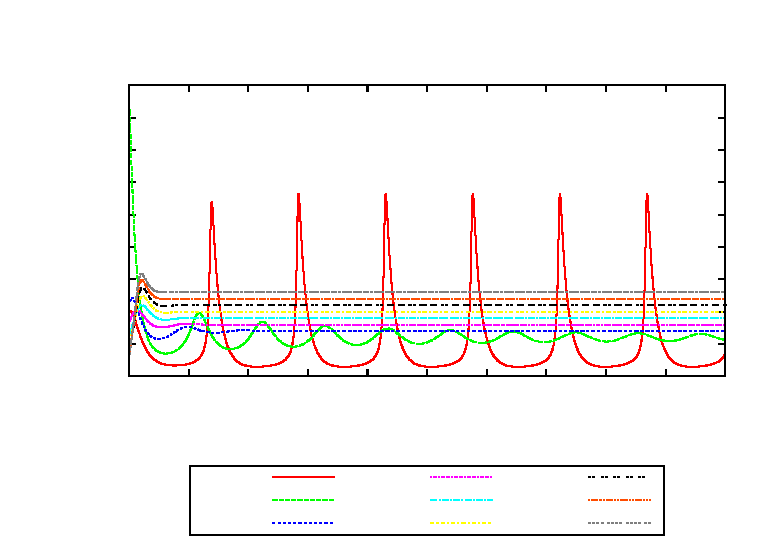
\includegraphics{b04u1v1}}%
    \gplfronttext
  \end{picture}%
\endgroup

\caption{b04}\label{b04u1v1}
\end{figure}
\begin{figure}
\centering
% GNUPLOT: LaTeX picture with Postscript
\begingroup
  \makeatletter
  \providecommand\color[2][]{%
    \GenericError{(gnuplot) \space\space\space\@spaces}{%
      Package color not loaded in conjunction with
      terminal option `colourtext'%
    }{See the gnuplot documentation for explanation.%
    }{Either use 'blacktext' in gnuplot or load the package
      color.sty in LaTeX.}%
    \renewcommand\color[2][]{}%
  }%
  \providecommand\includegraphics[2][]{%
    \GenericError{(gnuplot) \space\space\space\@spaces}{%
      Package graphicx or graphics not loaded%
    }{See the gnuplot documentation for explanation.%
    }{The gnuplot epslatex terminal needs graphicx.sty or graphics.sty.}%
    \renewcommand\includegraphics[2][]{}%
  }%
  \providecommand\rotatebox[2]{#2}%
  \@ifundefined{ifGPcolor}{%
    \newif\ifGPcolor
    \GPcolortrue
  }{}%
  \@ifundefined{ifGPblacktext}{%
    \newif\ifGPblacktext
    \GPblacktexttrue
  }{}%
  % define a \g@addto@macro without @ in the name:
  \let\gplgaddtomacro\g@addto@macro
  % define empty templates for all commands taking text:
  \gdef\gplbacktext{}%
  \gdef\gplfronttext{}%
  \makeatother
  \ifGPblacktext
    % no textcolor at all
    \def\colorrgb#1{}%
    \def\colorgray#1{}%
  \else
    % gray or color?
    \ifGPcolor
      \def\colorrgb#1{\color[rgb]{#1}}%
      \def\colorgray#1{\color[gray]{#1}}%
      \expandafter\def\csname LTw\endcsname{\color{white}}%
      \expandafter\def\csname LTb\endcsname{\color{black}}%
      \expandafter\def\csname LTa\endcsname{\color{black}}%
      \expandafter\def\csname LT0\endcsname{\color[rgb]{1,0,0}}%
      \expandafter\def\csname LT1\endcsname{\color[rgb]{0,1,0}}%
      \expandafter\def\csname LT2\endcsname{\color[rgb]{0,0,1}}%
      \expandafter\def\csname LT3\endcsname{\color[rgb]{1,0,1}}%
      \expandafter\def\csname LT4\endcsname{\color[rgb]{0,1,1}}%
      \expandafter\def\csname LT5\endcsname{\color[rgb]{1,1,0}}%
      \expandafter\def\csname LT6\endcsname{\color[rgb]{0,0,0}}%
      \expandafter\def\csname LT7\endcsname{\color[rgb]{1,0.3,0}}%
      \expandafter\def\csname LT8\endcsname{\color[rgb]{0.5,0.5,0.5}}%
    \else
      % gray
      \def\colorrgb#1{\color{black}}%
      \def\colorgray#1{\color[gray]{#1}}%
      \expandafter\def\csname LTw\endcsname{\color{white}}%
      \expandafter\def\csname LTb\endcsname{\color{black}}%
      \expandafter\def\csname LTa\endcsname{\color{black}}%
      \expandafter\def\csname LT0\endcsname{\color{black}}%
      \expandafter\def\csname LT1\endcsname{\color{black}}%
      \expandafter\def\csname LT2\endcsname{\color{black}}%
      \expandafter\def\csname LT3\endcsname{\color{black}}%
      \expandafter\def\csname LT4\endcsname{\color{black}}%
      \expandafter\def\csname LT5\endcsname{\color{black}}%
      \expandafter\def\csname LT6\endcsname{\color{black}}%
      \expandafter\def\csname LT7\endcsname{\color{black}}%
      \expandafter\def\csname LT8\endcsname{\color{black}}%
    \fi
  \fi
  \setlength{\unitlength}{0.0500bp}%
  \begin{picture}(7200.00,5040.00)%
    \gplgaddtomacro\gplbacktext{%
      \csname LTb\endcsname%
      \put(946,1584){\makebox(0,0)[r]{\strut{} 0}}%
      \put(946,1933){\makebox(0,0)[r]{\strut{} 0.5}}%
      \put(946,2283){\makebox(0,0)[r]{\strut{} 1}}%
      \put(946,2632){\makebox(0,0)[r]{\strut{} 1.5}}%
      \put(946,2982){\makebox(0,0)[r]{\strut{} 2}}%
      \put(946,3331){\makebox(0,0)[r]{\strut{} 2.5}}%
      \put(946,3680){\makebox(0,0)[r]{\strut{} 3}}%
      \put(946,4030){\makebox(0,0)[r]{\strut{} 3.5}}%
      \put(946,4379){\makebox(0,0)[r]{\strut{} 4}}%
      \put(1078,1364){\makebox(0,0){\strut{} 0}}%
      \put(1651,1364){\makebox(0,0){\strut{} 10}}%
      \put(2223,1364){\makebox(0,0){\strut{} 20}}%
      \put(2796,1364){\makebox(0,0){\strut{} 30}}%
      \put(3368,1364){\makebox(0,0){\strut{} 40}}%
      \put(3941,1364){\makebox(0,0){\strut{} 50}}%
      \put(4513,1364){\makebox(0,0){\strut{} 60}}%
      \put(5086,1364){\makebox(0,0){\strut{} 70}}%
      \put(5658,1364){\makebox(0,0){\strut{} 80}}%
      \put(6231,1364){\makebox(0,0){\strut{} 90}}%
      \put(6803,1364){\makebox(0,0){\strut{} 100}}%
      \put(176,2981){\rotatebox{-270}{\makebox(0,0){\strut{}Dichte $v$}}}%
      \put(3940,1034){\makebox(0,0){\strut{}Zeit $t$}}%
      \put(3940,4709){\makebox(0,0){\strut{}Parameter: $a=0.1 \, ...\, 0.9, b=0.4, u_0=v_0=1$ bei einer Schrittweite von $\Delta t=0.001$}}%
    }%
    \gplgaddtomacro\gplfronttext{%
      \csname LTb\endcsname%
      \put(2328,613){\makebox(0,0)[r]{\strut{}a=0.1}}%
      \csname LTb\endcsname%
      \put(2328,393){\makebox(0,0)[r]{\strut{}a=0.2}}%
      \csname LTb\endcsname%
      \put(2328,173){\makebox(0,0)[r]{\strut{}a=0.3}}%
      \csname LTb\endcsname%
      \put(3843,613){\makebox(0,0)[r]{\strut{}a=0.4}}%
      \csname LTb\endcsname%
      \put(3843,393){\makebox(0,0)[r]{\strut{}a=0.5}}%
      \csname LTb\endcsname%
      \put(3843,173){\makebox(0,0)[r]{\strut{}a=0.6}}%
      \csname LTb\endcsname%
      \put(5358,613){\makebox(0,0)[r]{\strut{}a=0.4}}%
      \csname LTb\endcsname%
      \put(5358,393){\makebox(0,0)[r]{\strut{}a=0.8}}%
      \csname LTb\endcsname%
      \put(5358,173){\makebox(0,0)[r]{\strut{}a=0.9}}%
    }%
    \gplbacktext
    \put(0,0){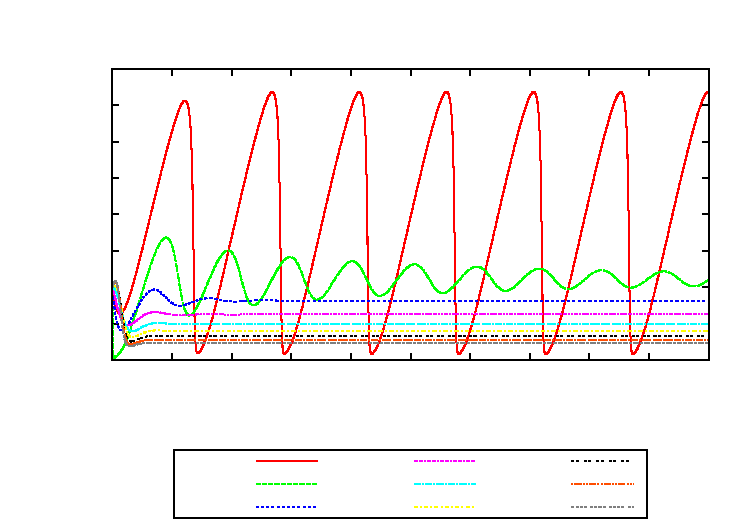
\includegraphics{b04u1v1v}}%
    \gplfronttext
  \end{picture}%
\endgroup

\caption{b04v}\label{b04u1v1v}
\end{figure}
\begin{figure}
\centering
% GNUPLOT: LaTeX picture with Postscript
\begingroup
  \makeatletter
  \providecommand\color[2][]{%
    \GenericError{(gnuplot) \space\space\space\@spaces}{%
      Package color not loaded in conjunction with
      terminal option `colourtext'%
    }{See the gnuplot documentation for explanation.%
    }{Either use 'blacktext' in gnuplot or load the package
      color.sty in LaTeX.}%
    \renewcommand\color[2][]{}%
  }%
  \providecommand\includegraphics[2][]{%
    \GenericError{(gnuplot) \space\space\space\@spaces}{%
      Package graphicx or graphics not loaded%
    }{See the gnuplot documentation for explanation.%
    }{The gnuplot epslatex terminal needs graphicx.sty or graphics.sty.}%
    \renewcommand\includegraphics[2][]{}%
  }%
  \providecommand\rotatebox[2]{#2}%
  \@ifundefined{ifGPcolor}{%
    \newif\ifGPcolor
    \GPcolortrue
  }{}%
  \@ifundefined{ifGPblacktext}{%
    \newif\ifGPblacktext
    \GPblacktexttrue
  }{}%
  % define a \g@addto@macro without @ in the name:
  \let\gplgaddtomacro\g@addto@macro
  % define empty templates for all commands taking text:
  \gdef\gplbacktext{}%
  \gdef\gplfronttext{}%
  \makeatother
  \ifGPblacktext
    % no textcolor at all
    \def\colorrgb#1{}%
    \def\colorgray#1{}%
  \else
    % gray or color?
    \ifGPcolor
      \def\colorrgb#1{\color[rgb]{#1}}%
      \def\colorgray#1{\color[gray]{#1}}%
      \expandafter\def\csname LTw\endcsname{\color{white}}%
      \expandafter\def\csname LTb\endcsname{\color{black}}%
      \expandafter\def\csname LTa\endcsname{\color{black}}%
      \expandafter\def\csname LT0\endcsname{\color[rgb]{1,0,0}}%
      \expandafter\def\csname LT1\endcsname{\color[rgb]{0,1,0}}%
      \expandafter\def\csname LT2\endcsname{\color[rgb]{0,0,1}}%
      \expandafter\def\csname LT3\endcsname{\color[rgb]{1,0,1}}%
      \expandafter\def\csname LT4\endcsname{\color[rgb]{0,1,1}}%
      \expandafter\def\csname LT5\endcsname{\color[rgb]{1,1,0}}%
      \expandafter\def\csname LT6\endcsname{\color[rgb]{0,0,0}}%
      \expandafter\def\csname LT7\endcsname{\color[rgb]{1,0.3,0}}%
      \expandafter\def\csname LT8\endcsname{\color[rgb]{0.5,0.5,0.5}}%
    \else
      % gray
      \def\colorrgb#1{\color{black}}%
      \def\colorgray#1{\color[gray]{#1}}%
      \expandafter\def\csname LTw\endcsname{\color{white}}%
      \expandafter\def\csname LTb\endcsname{\color{black}}%
      \expandafter\def\csname LTa\endcsname{\color{black}}%
      \expandafter\def\csname LT0\endcsname{\color{black}}%
      \expandafter\def\csname LT1\endcsname{\color{black}}%
      \expandafter\def\csname LT2\endcsname{\color{black}}%
      \expandafter\def\csname LT3\endcsname{\color{black}}%
      \expandafter\def\csname LT4\endcsname{\color{black}}%
      \expandafter\def\csname LT5\endcsname{\color{black}}%
      \expandafter\def\csname LT6\endcsname{\color{black}}%
      \expandafter\def\csname LT7\endcsname{\color{black}}%
      \expandafter\def\csname LT8\endcsname{\color{black}}%
    \fi
  \fi
  \setlength{\unitlength}{0.0500bp}%
  \begin{picture}(7200.00,5040.00)%
    \gplgaddtomacro\gplbacktext{%
      \csname LTb\endcsname%
      \put(946,1584){\makebox(0,0)[r]{\strut{} 0}}%
      \put(946,1933){\makebox(0,0)[r]{\strut{} 0.5}}%
      \put(946,2283){\makebox(0,0)[r]{\strut{} 1}}%
      \put(946,2632){\makebox(0,0)[r]{\strut{} 1.5}}%
      \put(946,2982){\makebox(0,0)[r]{\strut{} 2}}%
      \put(946,3331){\makebox(0,0)[r]{\strut{} 2.5}}%
      \put(946,3680){\makebox(0,0)[r]{\strut{} 3}}%
      \put(946,4030){\makebox(0,0)[r]{\strut{} 3.5}}%
      \put(946,4379){\makebox(0,0)[r]{\strut{} 4}}%
      \put(1078,1364){\makebox(0,0){\strut{} 0}}%
      \put(1714,1364){\makebox(0,0){\strut{} 0.5}}%
      \put(2350,1364){\makebox(0,0){\strut{} 1}}%
      \put(2986,1364){\makebox(0,0){\strut{} 1.5}}%
      \put(3622,1364){\makebox(0,0){\strut{} 2}}%
      \put(4259,1364){\makebox(0,0){\strut{} 2.5}}%
      \put(4895,1364){\makebox(0,0){\strut{} 3}}%
      \put(5531,1364){\makebox(0,0){\strut{} 3.5}}%
      \put(6167,1364){\makebox(0,0){\strut{} 4}}%
      \put(6803,1364){\makebox(0,0){\strut{} 4.5}}%
      \put(176,2981){\rotatebox{-270}{\makebox(0,0){\strut{}Dichte $v$}}}%
      \put(3940,1034){\makebox(0,0){\strut{}Dichte $u$}}%
      \put(3940,4709){\makebox(0,0){\strut{}Parameter: $a=0.1 \, ...\, 0.9, b=0.4, u_0=v_0=1$ bei einer Schrittweite von $\Delta t=0.001$}}%
    }%
    \gplgaddtomacro\gplfronttext{%
      \csname LTb\endcsname%
      \put(2328,613){\makebox(0,0)[r]{\strut{}a=0.1}}%
      \csname LTb\endcsname%
      \put(2328,393){\makebox(0,0)[r]{\strut{}a=0.2}}%
      \csname LTb\endcsname%
      \put(2328,173){\makebox(0,0)[r]{\strut{}a=0.3}}%
      \csname LTb\endcsname%
      \put(3843,613){\makebox(0,0)[r]{\strut{}a=0.4}}%
      \csname LTb\endcsname%
      \put(3843,393){\makebox(0,0)[r]{\strut{}a=0.5}}%
      \csname LTb\endcsname%
      \put(3843,173){\makebox(0,0)[r]{\strut{}a=0.6}}%
      \csname LTb\endcsname%
      \put(5358,613){\makebox(0,0)[r]{\strut{}a=0.4}}%
      \csname LTb\endcsname%
      \put(5358,393){\makebox(0,0)[r]{\strut{}a=0.8}}%
      \csname LTb\endcsname%
      \put(5358,173){\makebox(0,0)[r]{\strut{}a=0.9}}%
    }%
    \gplbacktext
    \put(0,0){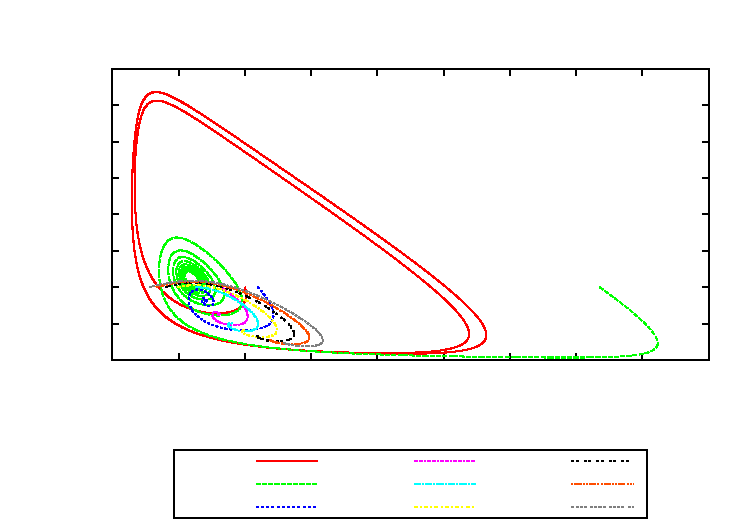
\includegraphics{b04u1v1uv}}%
    \gplfronttext
  \end{picture}%
\endgroup

\caption{b04uv}\label{b04u1v1uv}
\end{figure}
\begin{figure}
\centering
% GNUPLOT: LaTeX picture with Postscript
\begingroup
  \makeatletter
  \providecommand\color[2][]{%
    \GenericError{(gnuplot) \space\space\space\@spaces}{%
      Package color not loaded in conjunction with
      terminal option `colourtext'%
    }{See the gnuplot documentation for explanation.%
    }{Either use 'blacktext' in gnuplot or load the package
      color.sty in LaTeX.}%
    \renewcommand\color[2][]{}%
  }%
  \providecommand\includegraphics[2][]{%
    \GenericError{(gnuplot) \space\space\space\@spaces}{%
      Package graphicx or graphics not loaded%
    }{See the gnuplot documentation for explanation.%
    }{The gnuplot epslatex terminal needs graphicx.sty or graphics.sty.}%
    \renewcommand\includegraphics[2][]{}%
  }%
  \providecommand\rotatebox[2]{#2}%
  \@ifundefined{ifGPcolor}{%
    \newif\ifGPcolor
    \GPcolortrue
  }{}%
  \@ifundefined{ifGPblacktext}{%
    \newif\ifGPblacktext
    \GPblacktexttrue
  }{}%
  % define a \g@addto@macro without @ in the name:
  \let\gplgaddtomacro\g@addto@macro
  % define empty templates for all commands taking text:
  \gdef\gplbacktext{}%
  \gdef\gplfronttext{}%
  \makeatother
  \ifGPblacktext
    % no textcolor at all
    \def\colorrgb#1{}%
    \def\colorgray#1{}%
  \else
    % gray or color?
    \ifGPcolor
      \def\colorrgb#1{\color[rgb]{#1}}%
      \def\colorgray#1{\color[gray]{#1}}%
      \expandafter\def\csname LTw\endcsname{\color{white}}%
      \expandafter\def\csname LTb\endcsname{\color{black}}%
      \expandafter\def\csname LTa\endcsname{\color{black}}%
      \expandafter\def\csname LT0\endcsname{\color[rgb]{1,0,0}}%
      \expandafter\def\csname LT1\endcsname{\color[rgb]{0,1,0}}%
      \expandafter\def\csname LT2\endcsname{\color[rgb]{0,0,1}}%
      \expandafter\def\csname LT3\endcsname{\color[rgb]{1,0,1}}%
      \expandafter\def\csname LT4\endcsname{\color[rgb]{0,1,1}}%
      \expandafter\def\csname LT5\endcsname{\color[rgb]{1,1,0}}%
      \expandafter\def\csname LT6\endcsname{\color[rgb]{0,0,0}}%
      \expandafter\def\csname LT7\endcsname{\color[rgb]{1,0.3,0}}%
      \expandafter\def\csname LT8\endcsname{\color[rgb]{0.5,0.5,0.5}}%
    \else
      % gray
      \def\colorrgb#1{\color{black}}%
      \def\colorgray#1{\color[gray]{#1}}%
      \expandafter\def\csname LTw\endcsname{\color{white}}%
      \expandafter\def\csname LTb\endcsname{\color{black}}%
      \expandafter\def\csname LTa\endcsname{\color{black}}%
      \expandafter\def\csname LT0\endcsname{\color{black}}%
      \expandafter\def\csname LT1\endcsname{\color{black}}%
      \expandafter\def\csname LT2\endcsname{\color{black}}%
      \expandafter\def\csname LT3\endcsname{\color{black}}%
      \expandafter\def\csname LT4\endcsname{\color{black}}%
      \expandafter\def\csname LT5\endcsname{\color{black}}%
      \expandafter\def\csname LT6\endcsname{\color{black}}%
      \expandafter\def\csname LT7\endcsname{\color{black}}%
      \expandafter\def\csname LT8\endcsname{\color{black}}%
    \fi
  \fi
  \setlength{\unitlength}{0.0500bp}%
  \begin{picture}(7200.00,5040.00)%
    \gplgaddtomacro\gplbacktext{%
      \csname LTb\endcsname%
      \put(946,1584){\makebox(0,0)[r]{\strut{} 0.2}}%
      \put(946,1895){\makebox(0,0)[r]{\strut{} 0.4}}%
      \put(946,2205){\makebox(0,0)[r]{\strut{} 0.6}}%
      \put(946,2516){\makebox(0,0)[r]{\strut{} 0.8}}%
      \put(946,2826){\makebox(0,0)[r]{\strut{} 1}}%
      \put(946,3137){\makebox(0,0)[r]{\strut{} 1.2}}%
      \put(946,3447){\makebox(0,0)[r]{\strut{} 1.4}}%
      \put(946,3758){\makebox(0,0)[r]{\strut{} 1.6}}%
      \put(946,4068){\makebox(0,0)[r]{\strut{} 1.8}}%
      \put(946,4379){\makebox(0,0)[r]{\strut{} 2}}%
      \put(1078,1364){\makebox(0,0){\strut{} 0}}%
      \put(1651,1364){\makebox(0,0){\strut{} 10}}%
      \put(2223,1364){\makebox(0,0){\strut{} 20}}%
      \put(2796,1364){\makebox(0,0){\strut{} 30}}%
      \put(3368,1364){\makebox(0,0){\strut{} 40}}%
      \put(3941,1364){\makebox(0,0){\strut{} 50}}%
      \put(4513,1364){\makebox(0,0){\strut{} 60}}%
      \put(5086,1364){\makebox(0,0){\strut{} 70}}%
      \put(5658,1364){\makebox(0,0){\strut{} 80}}%
      \put(6231,1364){\makebox(0,0){\strut{} 90}}%
      \put(6803,1364){\makebox(0,0){\strut{} 100}}%
      \put(176,2981){\rotatebox{-270}{\makebox(0,0){\strut{}Dichte $u$}}}%
      \put(3940,1034){\makebox(0,0){\strut{}Zeit $t$}}%
      \put(3940,4709){\makebox(0,0){\strut{}Parameter: $a=0.1 \, ...\, 0.9, b=0.7, u_0=v_0=1$ bei einer Schrittweite von $\Delta t=0.001$}}%
    }%
    \gplgaddtomacro\gplfronttext{%
      \csname LTb\endcsname%
      \put(2328,613){\makebox(0,0)[r]{\strut{}a=0.1}}%
      \csname LTb\endcsname%
      \put(2328,393){\makebox(0,0)[r]{\strut{}a=0.2}}%
      \csname LTb\endcsname%
      \put(2328,173){\makebox(0,0)[r]{\strut{}a=0.3}}%
      \csname LTb\endcsname%
      \put(3843,613){\makebox(0,0)[r]{\strut{}a=0.4}}%
      \csname LTb\endcsname%
      \put(3843,393){\makebox(0,0)[r]{\strut{}a=0.5}}%
      \csname LTb\endcsname%
      \put(3843,173){\makebox(0,0)[r]{\strut{}a=0.6}}%
      \csname LTb\endcsname%
      \put(5358,613){\makebox(0,0)[r]{\strut{}a=0.7}}%
      \csname LTb\endcsname%
      \put(5358,393){\makebox(0,0)[r]{\strut{}a=0.8}}%
      \csname LTb\endcsname%
      \put(5358,173){\makebox(0,0)[r]{\strut{}a=0.9}}%
    }%
    \gplbacktext
    \put(0,0){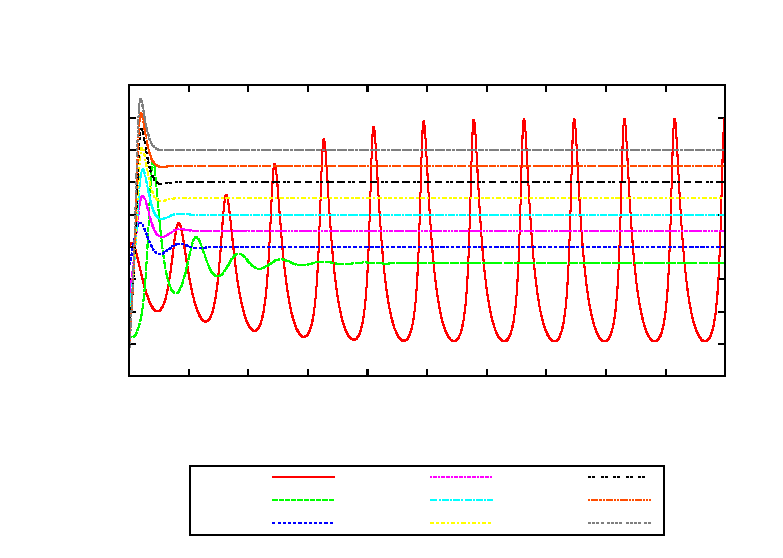
\includegraphics{b07u1v1}}%
    \gplfronttext
  \end{picture}%
\endgroup

\caption{b07\label{b07u1v1}}
\end{figure}
\begin{figure}
\centering
% GNUPLOT: LaTeX picture with Postscript
\begingroup
  \makeatletter
  \providecommand\color[2][]{%
    \GenericError{(gnuplot) \space\space\space\@spaces}{%
      Package color not loaded in conjunction with
      terminal option `colourtext'%
    }{See the gnuplot documentation for explanation.%
    }{Either use 'blacktext' in gnuplot or load the package
      color.sty in LaTeX.}%
    \renewcommand\color[2][]{}%
  }%
  \providecommand\includegraphics[2][]{%
    \GenericError{(gnuplot) \space\space\space\@spaces}{%
      Package graphicx or graphics not loaded%
    }{See the gnuplot documentation for explanation.%
    }{The gnuplot epslatex terminal needs graphicx.sty or graphics.sty.}%
    \renewcommand\includegraphics[2][]{}%
  }%
  \providecommand\rotatebox[2]{#2}%
  \@ifundefined{ifGPcolor}{%
    \newif\ifGPcolor
    \GPcolortrue
  }{}%
  \@ifundefined{ifGPblacktext}{%
    \newif\ifGPblacktext
    \GPblacktexttrue
  }{}%
  % define a \g@addto@macro without @ in the name:
  \let\gplgaddtomacro\g@addto@macro
  % define empty templates for all commands taking text:
  \gdef\gplbacktext{}%
  \gdef\gplfronttext{}%
  \makeatother
  \ifGPblacktext
    % no textcolor at all
    \def\colorrgb#1{}%
    \def\colorgray#1{}%
  \else
    % gray or color?
    \ifGPcolor
      \def\colorrgb#1{\color[rgb]{#1}}%
      \def\colorgray#1{\color[gray]{#1}}%
      \expandafter\def\csname LTw\endcsname{\color{white}}%
      \expandafter\def\csname LTb\endcsname{\color{black}}%
      \expandafter\def\csname LTa\endcsname{\color{black}}%
      \expandafter\def\csname LT0\endcsname{\color[rgb]{1,0,0}}%
      \expandafter\def\csname LT1\endcsname{\color[rgb]{0,1,0}}%
      \expandafter\def\csname LT2\endcsname{\color[rgb]{0,0,1}}%
      \expandafter\def\csname LT3\endcsname{\color[rgb]{1,0,1}}%
      \expandafter\def\csname LT4\endcsname{\color[rgb]{0,1,1}}%
      \expandafter\def\csname LT5\endcsname{\color[rgb]{1,1,0}}%
      \expandafter\def\csname LT6\endcsname{\color[rgb]{0,0,0}}%
      \expandafter\def\csname LT7\endcsname{\color[rgb]{1,0.3,0}}%
      \expandafter\def\csname LT8\endcsname{\color[rgb]{0.5,0.5,0.5}}%
    \else
      % gray
      \def\colorrgb#1{\color{black}}%
      \def\colorgray#1{\color[gray]{#1}}%
      \expandafter\def\csname LTw\endcsname{\color{white}}%
      \expandafter\def\csname LTb\endcsname{\color{black}}%
      \expandafter\def\csname LTa\endcsname{\color{black}}%
      \expandafter\def\csname LT0\endcsname{\color{black}}%
      \expandafter\def\csname LT1\endcsname{\color{black}}%
      \expandafter\def\csname LT2\endcsname{\color{black}}%
      \expandafter\def\csname LT3\endcsname{\color{black}}%
      \expandafter\def\csname LT4\endcsname{\color{black}}%
      \expandafter\def\csname LT5\endcsname{\color{black}}%
      \expandafter\def\csname LT6\endcsname{\color{black}}%
      \expandafter\def\csname LT7\endcsname{\color{black}}%
      \expandafter\def\csname LT8\endcsname{\color{black}}%
    \fi
  \fi
  \setlength{\unitlength}{0.0500bp}%
  \begin{picture}(7200.00,5040.00)%
    \gplgaddtomacro\gplbacktext{%
      \csname LTb\endcsname%
      \put(946,1584){\makebox(0,0)[r]{\strut{} 0}}%
      \put(946,2143){\makebox(0,0)[r]{\strut{} 0.5}}%
      \put(946,2702){\makebox(0,0)[r]{\strut{} 1}}%
      \put(946,3261){\makebox(0,0)[r]{\strut{} 1.5}}%
      \put(946,3820){\makebox(0,0)[r]{\strut{} 2}}%
      \put(946,4379){\makebox(0,0)[r]{\strut{} 2.5}}%
      \put(1078,1364){\makebox(0,0){\strut{} 0}}%
      \put(1651,1364){\makebox(0,0){\strut{} 10}}%
      \put(2223,1364){\makebox(0,0){\strut{} 20}}%
      \put(2796,1364){\makebox(0,0){\strut{} 30}}%
      \put(3368,1364){\makebox(0,0){\strut{} 40}}%
      \put(3941,1364){\makebox(0,0){\strut{} 50}}%
      \put(4513,1364){\makebox(0,0){\strut{} 60}}%
      \put(5086,1364){\makebox(0,0){\strut{} 70}}%
      \put(5658,1364){\makebox(0,0){\strut{} 80}}%
      \put(6231,1364){\makebox(0,0){\strut{} 90}}%
      \put(6803,1364){\makebox(0,0){\strut{} 100}}%
      \put(176,2981){\rotatebox{-270}{\makebox(0,0){\strut{}Dichte $v$}}}%
      \put(3940,1034){\makebox(0,0){\strut{}Zeit $t$}}%
      \put(3940,4709){\makebox(0,0){\strut{}Parameter: $a=0.1 \, ...\, 0.9, b=0.7, u_0=v_0=1$ bei einer Schrittweite von $\Delta t=0.001$}}%
    }%
    \gplgaddtomacro\gplfronttext{%
      \csname LTb\endcsname%
      \put(2328,613){\makebox(0,0)[r]{\strut{}a=0.1}}%
      \csname LTb\endcsname%
      \put(2328,393){\makebox(0,0)[r]{\strut{}a=0.2}}%
      \csname LTb\endcsname%
      \put(2328,173){\makebox(0,0)[r]{\strut{}a=0.3}}%
      \csname LTb\endcsname%
      \put(3843,613){\makebox(0,0)[r]{\strut{}a=0.4}}%
      \csname LTb\endcsname%
      \put(3843,393){\makebox(0,0)[r]{\strut{}a=0.5}}%
      \csname LTb\endcsname%
      \put(3843,173){\makebox(0,0)[r]{\strut{}a=0.6}}%
      \csname LTb\endcsname%
      \put(5358,613){\makebox(0,0)[r]{\strut{}a=0.7}}%
      \csname LTb\endcsname%
      \put(5358,393){\makebox(0,0)[r]{\strut{}a=0.8}}%
      \csname LTb\endcsname%
      \put(5358,173){\makebox(0,0)[r]{\strut{}a=0.9}}%
    }%
    \gplbacktext
    \put(0,0){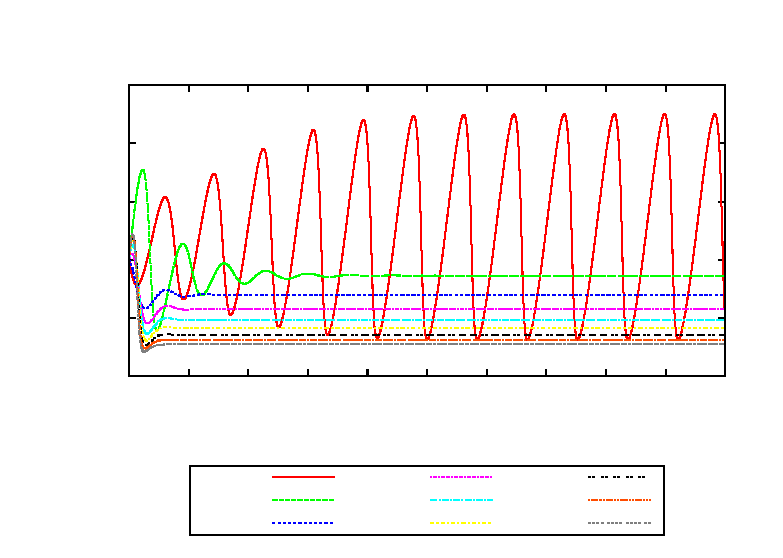
\includegraphics{b07u1v1v}}%
    \gplfronttext
  \end{picture}%
\endgroup

\caption{b07v\label{b07u1v1v}}
\end{figure}
\begin{figure}
\centering
% GNUPLOT: LaTeX picture with Postscript
\begingroup
  \makeatletter
  \providecommand\color[2][]{%
    \GenericError{(gnuplot) \space\space\space\@spaces}{%
      Package color not loaded in conjunction with
      terminal option `colourtext'%
    }{See the gnuplot documentation for explanation.%
    }{Either use 'blacktext' in gnuplot or load the package
      color.sty in LaTeX.}%
    \renewcommand\color[2][]{}%
  }%
  \providecommand\includegraphics[2][]{%
    \GenericError{(gnuplot) \space\space\space\@spaces}{%
      Package graphicx or graphics not loaded%
    }{See the gnuplot documentation for explanation.%
    }{The gnuplot epslatex terminal needs graphicx.sty or graphics.sty.}%
    \renewcommand\includegraphics[2][]{}%
  }%
  \providecommand\rotatebox[2]{#2}%
  \@ifundefined{ifGPcolor}{%
    \newif\ifGPcolor
    \GPcolortrue
  }{}%
  \@ifundefined{ifGPblacktext}{%
    \newif\ifGPblacktext
    \GPblacktexttrue
  }{}%
  % define a \g@addto@macro without @ in the name:
  \let\gplgaddtomacro\g@addto@macro
  % define empty templates for all commands taking text:
  \gdef\gplbacktext{}%
  \gdef\gplfronttext{}%
  \makeatother
  \ifGPblacktext
    % no textcolor at all
    \def\colorrgb#1{}%
    \def\colorgray#1{}%
  \else
    % gray or color?
    \ifGPcolor
      \def\colorrgb#1{\color[rgb]{#1}}%
      \def\colorgray#1{\color[gray]{#1}}%
      \expandafter\def\csname LTw\endcsname{\color{white}}%
      \expandafter\def\csname LTb\endcsname{\color{black}}%
      \expandafter\def\csname LTa\endcsname{\color{black}}%
      \expandafter\def\csname LT0\endcsname{\color[rgb]{1,0,0}}%
      \expandafter\def\csname LT1\endcsname{\color[rgb]{0,1,0}}%
      \expandafter\def\csname LT2\endcsname{\color[rgb]{0,0,1}}%
      \expandafter\def\csname LT3\endcsname{\color[rgb]{1,0,1}}%
      \expandafter\def\csname LT4\endcsname{\color[rgb]{0,1,1}}%
      \expandafter\def\csname LT5\endcsname{\color[rgb]{1,1,0}}%
      \expandafter\def\csname LT6\endcsname{\color[rgb]{0,0,0}}%
      \expandafter\def\csname LT7\endcsname{\color[rgb]{1,0.3,0}}%
      \expandafter\def\csname LT8\endcsname{\color[rgb]{0.5,0.5,0.5}}%
    \else
      % gray
      \def\colorrgb#1{\color{black}}%
      \def\colorgray#1{\color[gray]{#1}}%
      \expandafter\def\csname LTw\endcsname{\color{white}}%
      \expandafter\def\csname LTb\endcsname{\color{black}}%
      \expandafter\def\csname LTa\endcsname{\color{black}}%
      \expandafter\def\csname LT0\endcsname{\color{black}}%
      \expandafter\def\csname LT1\endcsname{\color{black}}%
      \expandafter\def\csname LT2\endcsname{\color{black}}%
      \expandafter\def\csname LT3\endcsname{\color{black}}%
      \expandafter\def\csname LT4\endcsname{\color{black}}%
      \expandafter\def\csname LT5\endcsname{\color{black}}%
      \expandafter\def\csname LT6\endcsname{\color{black}}%
      \expandafter\def\csname LT7\endcsname{\color{black}}%
      \expandafter\def\csname LT8\endcsname{\color{black}}%
    \fi
  \fi
  \setlength{\unitlength}{0.0500bp}%
  \begin{picture}(7200.00,5040.00)%
    \gplgaddtomacro\gplbacktext{%
      \csname LTb\endcsname%
      \put(946,1584){\makebox(0,0)[r]{\strut{} 0}}%
      \put(946,2143){\makebox(0,0)[r]{\strut{} 0.5}}%
      \put(946,2702){\makebox(0,0)[r]{\strut{} 1}}%
      \put(946,3261){\makebox(0,0)[r]{\strut{} 1.5}}%
      \put(946,3820){\makebox(0,0)[r]{\strut{} 2}}%
      \put(946,4379){\makebox(0,0)[r]{\strut{} 2.5}}%
      \put(1078,1364){\makebox(0,0){\strut{} 0.2}}%
      \put(1714,1364){\makebox(0,0){\strut{} 0.4}}%
      \put(2350,1364){\makebox(0,0){\strut{} 0.6}}%
      \put(2986,1364){\makebox(0,0){\strut{} 0.8}}%
      \put(3622,1364){\makebox(0,0){\strut{} 1}}%
      \put(4259,1364){\makebox(0,0){\strut{} 1.2}}%
      \put(4895,1364){\makebox(0,0){\strut{} 1.4}}%
      \put(5531,1364){\makebox(0,0){\strut{} 1.6}}%
      \put(6167,1364){\makebox(0,0){\strut{} 1.8}}%
      \put(6803,1364){\makebox(0,0){\strut{} 2}}%
      \put(176,2981){\rotatebox{-270}{\makebox(0,0){\strut{}Dichte $v$}}}%
      \put(3940,1034){\makebox(0,0){\strut{}Dichte $u$}}%
      \put(3940,4709){\makebox(0,0){\strut{}Parameter: $a=0.1 \, ...\, 0.9, b=0.7, u_0=v_0=1$ bei einer Schrittweite von $\Delta t=0.001$}}%
    }%
    \gplgaddtomacro\gplfronttext{%
      \csname LTb\endcsname%
      \put(2328,613){\makebox(0,0)[r]{\strut{}a=0.1}}%
      \csname LTb\endcsname%
      \put(2328,393){\makebox(0,0)[r]{\strut{}a=0.2}}%
      \csname LTb\endcsname%
      \put(2328,173){\makebox(0,0)[r]{\strut{}a=0.3}}%
      \csname LTb\endcsname%
      \put(3843,613){\makebox(0,0)[r]{\strut{}a=0.4}}%
      \csname LTb\endcsname%
      \put(3843,393){\makebox(0,0)[r]{\strut{}a=0.5}}%
      \csname LTb\endcsname%
      \put(3843,173){\makebox(0,0)[r]{\strut{}a=0.6}}%
      \csname LTb\endcsname%
      \put(5358,613){\makebox(0,0)[r]{\strut{}a=0.7}}%
      \csname LTb\endcsname%
      \put(5358,393){\makebox(0,0)[r]{\strut{}a=0.8}}%
      \csname LTb\endcsname%
      \put(5358,173){\makebox(0,0)[r]{\strut{}a=0.9}}%
    }%
    \gplbacktext
    \put(0,0){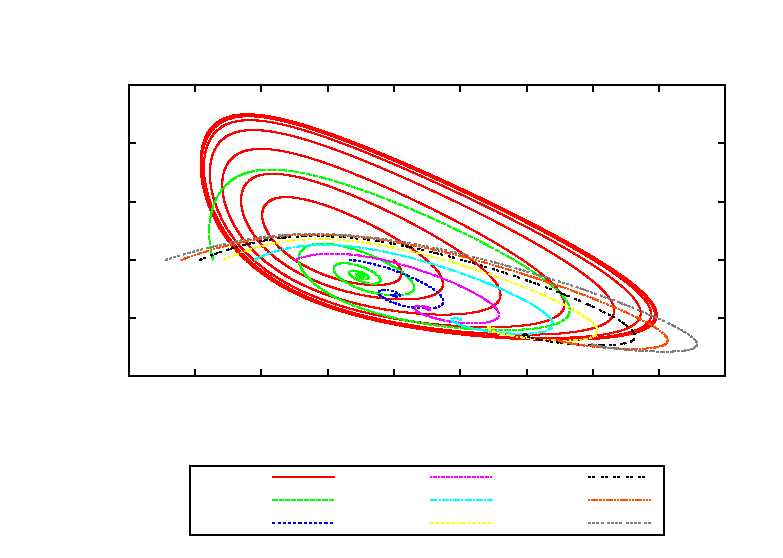
\includegraphics{b07u1v1uv}}%
    \gplfronttext
  \end{picture}%
\endgroup

\caption{b07uv}\label{b07u1v1uv}
\end{figure}


\section{Stabilität der Algorithmen}
Es ist keinesfalls belibig, welchen Algorithmus man verwendet.
Dies kann man insbesondere an der Abbildung \ref{fig:stabi} erkennen, welche in Teil a) für Schrittweiten von $\Delta t=0.1$ die Ergebnisse des Runge-Kutta-Algorithmus zu den Eingabewerten $a=0.01, b=0.99, u_0=v_0=1$ zeigt.
Hierbei ist eine  deutliche Konvergenz zu einem  Grenzwert von 1 erkennen.
Guckt man sich das zweite Bild an, welches zusätzlich noch für die selben Startwerte den Euler-Algorithmus auswertet, so erkennt man, dass komplett gegenteilige Aussagen entstehen.
Der grün dargestellte Euler-Algorithmus divergiert bis er konstante Schwingungen bei einer Amplitude von 1.2 ausführt.\\
Die Startwerte für diese Bilder habe ich durch wiederholtes Ausprobieren ermittelt, bis ein möglichst eindeutiges Bild entstand.

%%%%%%%%%%%%%%%%%%%%%%%%%%%%%%Größe um Abb nebeneinander%%%%%%%%%%%%%%%%%%%%%%%%%%%%%%
\begin{figure}[htb]
  \centering
   \subfigure[Runge-Kutta-Algorithmus 4. Ordnung\label{fig:stabirunge}]
   {% GNUPLOT: LaTeX picture with Postscript
\begingroup
  \makeatletter
  \providecommand\color[2][]{%
    \GenericError{(gnuplot) \space\space\space\@spaces}{%
      Package color not loaded in conjunction with
      terminal option `colourtext'%
    }{See the gnuplot documentation for explanation.%
    }{Either use 'blacktext' in gnuplot or load the package
      color.sty in LaTeX.}%
    \renewcommand\color[2][]{}%
  }%
  \providecommand\includegraphics[2][]{%
    \GenericError{(gnuplot) \space\space\space\@spaces}{%
      Package graphicx or graphics not loaded%
    }{See the gnuplot documentation for explanation.%
    }{The gnuplot epslatex terminal needs graphicx.sty or graphics.sty.}%
    \renewcommand\includegraphics[2][]{}%
  }%
  \providecommand\rotatebox[2]{#2}%
  \@ifundefined{ifGPcolor}{%
    \newif\ifGPcolor
    \GPcolortrue
  }{}%
  \@ifundefined{ifGPblacktext}{%
    \newif\ifGPblacktext
    \GPblacktexttrue
  }{}%
  % define a \g@addto@macro without @ in the name:
  \let\gplgaddtomacro\g@addto@macro
  % define empty templates for all commands taking text:
  \gdef\gplbacktext{}%
  \gdef\gplfronttext{}%
  \makeatother
  \ifGPblacktext
    % no textcolor at all
    \def\colorrgb#1{}%
    \def\colorgray#1{}%
  \else
    % gray or color?
    \ifGPcolor
      \def\colorrgb#1{\color[rgb]{#1}}%
      \def\colorgray#1{\color[gray]{#1}}%
      \expandafter\def\csname LTw\endcsname{\color{white}}%
      \expandafter\def\csname LTb\endcsname{\color{black}}%
      \expandafter\def\csname LTa\endcsname{\color{black}}%
      \expandafter\def\csname LT0\endcsname{\color[rgb]{1,0,0}}%
      \expandafter\def\csname LT1\endcsname{\color[rgb]{0,1,0}}%
      \expandafter\def\csname LT2\endcsname{\color[rgb]{0,0,1}}%
      \expandafter\def\csname LT3\endcsname{\color[rgb]{1,0,1}}%
      \expandafter\def\csname LT4\endcsname{\color[rgb]{0,1,1}}%
      \expandafter\def\csname LT5\endcsname{\color[rgb]{1,1,0}}%
      \expandafter\def\csname LT6\endcsname{\color[rgb]{0,0,0}}%
      \expandafter\def\csname LT7\endcsname{\color[rgb]{1,0.3,0}}%
      \expandafter\def\csname LT8\endcsname{\color[rgb]{0.5,0.5,0.5}}%
    \else
      % gray
      \def\colorrgb#1{\color{black}}%
      \def\colorgray#1{\color[gray]{#1}}%
      \expandafter\def\csname LTw\endcsname{\color{white}}%
      \expandafter\def\csname LTb\endcsname{\color{black}}%
      \expandafter\def\csname LTa\endcsname{\color{black}}%
      \expandafter\def\csname LT0\endcsname{\color{black}}%
      \expandafter\def\csname LT1\endcsname{\color{black}}%
      \expandafter\def\csname LT2\endcsname{\color{black}}%
      \expandafter\def\csname LT3\endcsname{\color{black}}%
      \expandafter\def\csname LT4\endcsname{\color{black}}%
      \expandafter\def\csname LT5\endcsname{\color{black}}%
      \expandafter\def\csname LT6\endcsname{\color{black}}%
      \expandafter\def\csname LT7\endcsname{\color{black}}%
      \expandafter\def\csname LT8\endcsname{\color{black}}%
    \fi
  \fi
  \setlength{\unitlength}{0.0500bp}%
  \begin{picture}(7200.00,5040.00)%
    \gplgaddtomacro\gplbacktext{%
      \csname LTb\endcsname%
      \put(1210,1144){\makebox(0,0)[r]{\strut{} 0.99}}%
      \put(1210,1468){\makebox(0,0)[r]{\strut{} 0.992}}%
      \put(1210,1791){\makebox(0,0)[r]{\strut{} 0.994}}%
      \put(1210,2115){\makebox(0,0)[r]{\strut{} 0.996}}%
      \put(1210,2438){\makebox(0,0)[r]{\strut{} 0.998}}%
      \put(1210,2762){\makebox(0,0)[r]{\strut{} 1}}%
      \put(1210,3085){\makebox(0,0)[r]{\strut{} 1.002}}%
      \put(1210,3409){\makebox(0,0)[r]{\strut{} 1.004}}%
      \put(1210,3732){\makebox(0,0)[r]{\strut{} 1.006}}%
      \put(1210,4056){\makebox(0,0)[r]{\strut{} 1.008}}%
      \put(1210,4379){\makebox(0,0)[r]{\strut{} 1.01}}%
      \put(1342,924){\makebox(0,0){\strut{} 0}}%
      \put(1888,924){\makebox(0,0){\strut{} 50}}%
      \put(2434,924){\makebox(0,0){\strut{} 100}}%
      \put(2980,924){\makebox(0,0){\strut{} 150}}%
      \put(3526,924){\makebox(0,0){\strut{} 200}}%
      \put(4073,924){\makebox(0,0){\strut{} 250}}%
      \put(4619,924){\makebox(0,0){\strut{} 300}}%
      \put(5165,924){\makebox(0,0){\strut{} 350}}%
      \put(5711,924){\makebox(0,0){\strut{} 400}}%
      \put(6257,924){\makebox(0,0){\strut{} 450}}%
      \put(6803,924){\makebox(0,0){\strut{} 500}}%
      \put(176,2761){\rotatebox{-270}{\makebox(0,0){\strut{}Dichte $u$}}}%
      \put(4072,594){\makebox(0,0){\strut{}Zeit $t$}}%
      \put(4072,4709){\makebox(0,0){\strut{}Parameter: $a=0.01, b=0.99, u_0=v_0=1$ bei einer Schrittweite von $\Delta t=0.1$}}%
    }%
    \gplgaddtomacro\gplfronttext{%
      \csname LTb\endcsname%
      \put(6153,173){\makebox(0,0)[r]{\strut{}Berechnung nach Runge-Kutta 4. Ordnung}}%
    }%
    \gplbacktext
    \put(0,0){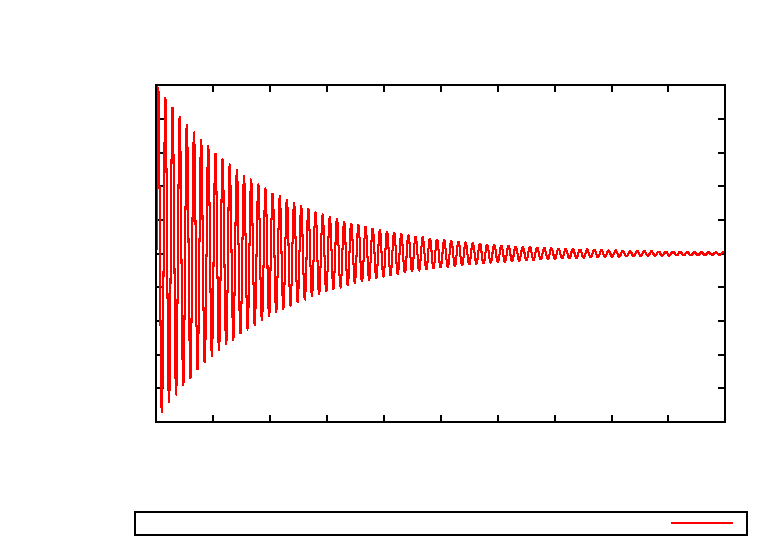
\includegraphics{a001b099uv1R}}%
    \gplfronttext
  \end{picture}%
\endgroup
}
   \hfill
   \subfigure[Vergleich Runge-Kutta-Algorithmus mit Euler bei identischen Randbedingungen\label{fig:stabibeide}]
   {% GNUPLOT: LaTeX picture with Postscript
\begingroup
  \makeatletter
  \providecommand\color[2][]{%
    \GenericError{(gnuplot) \space\space\space\@spaces}{%
      Package color not loaded in conjunction with
      terminal option `colourtext'%
    }{See the gnuplot documentation for explanation.%
    }{Either use 'blacktext' in gnuplot or load the package
      color.sty in LaTeX.}%
    \renewcommand\color[2][]{}%
  }%
  \providecommand\includegraphics[2][]{%
    \GenericError{(gnuplot) \space\space\space\@spaces}{%
      Package graphicx or graphics not loaded%
    }{See the gnuplot documentation for explanation.%
    }{The gnuplot epslatex terminal needs graphicx.sty or graphics.sty.}%
    \renewcommand\includegraphics[2][]{}%
  }%
  \providecommand\rotatebox[2]{#2}%
  \@ifundefined{ifGPcolor}{%
    \newif\ifGPcolor
    \GPcolortrue
  }{}%
  \@ifundefined{ifGPblacktext}{%
    \newif\ifGPblacktext
    \GPblacktexttrue
  }{}%
  % define a \g@addto@macro without @ in the name:
  \let\gplgaddtomacro\g@addto@macro
  % define empty templates for all commands taking text:
  \gdef\gplbacktext{}%
  \gdef\gplfronttext{}%
  \makeatother
  \ifGPblacktext
    % no textcolor at all
    \def\colorrgb#1{}%
    \def\colorgray#1{}%
  \else
    % gray or color?
    \ifGPcolor
      \def\colorrgb#1{\color[rgb]{#1}}%
      \def\colorgray#1{\color[gray]{#1}}%
      \expandafter\def\csname LTw\endcsname{\color{white}}%
      \expandafter\def\csname LTb\endcsname{\color{black}}%
      \expandafter\def\csname LTa\endcsname{\color{black}}%
      \expandafter\def\csname LT0\endcsname{\color[rgb]{1,0,0}}%
      \expandafter\def\csname LT1\endcsname{\color[rgb]{0,1,0}}%
      \expandafter\def\csname LT2\endcsname{\color[rgb]{0,0,1}}%
      \expandafter\def\csname LT3\endcsname{\color[rgb]{1,0,1}}%
      \expandafter\def\csname LT4\endcsname{\color[rgb]{0,1,1}}%
      \expandafter\def\csname LT5\endcsname{\color[rgb]{1,1,0}}%
      \expandafter\def\csname LT6\endcsname{\color[rgb]{0,0,0}}%
      \expandafter\def\csname LT7\endcsname{\color[rgb]{1,0.3,0}}%
      \expandafter\def\csname LT8\endcsname{\color[rgb]{0.5,0.5,0.5}}%
    \else
      % gray
      \def\colorrgb#1{\color{black}}%
      \def\colorgray#1{\color[gray]{#1}}%
      \expandafter\def\csname LTw\endcsname{\color{white}}%
      \expandafter\def\csname LTb\endcsname{\color{black}}%
      \expandafter\def\csname LTa\endcsname{\color{black}}%
      \expandafter\def\csname LT0\endcsname{\color{black}}%
      \expandafter\def\csname LT1\endcsname{\color{black}}%
      \expandafter\def\csname LT2\endcsname{\color{black}}%
      \expandafter\def\csname LT3\endcsname{\color{black}}%
      \expandafter\def\csname LT4\endcsname{\color{black}}%
      \expandafter\def\csname LT5\endcsname{\color{black}}%
      \expandafter\def\csname LT6\endcsname{\color{black}}%
      \expandafter\def\csname LT7\endcsname{\color{black}}%
      \expandafter\def\csname LT8\endcsname{\color{black}}%
    \fi
  \fi
  \setlength{\unitlength}{0.0500bp}%
  \begin{picture}(7200.00,5040.00)%
    \gplgaddtomacro\gplbacktext{%
      \csname LTb\endcsname%
      \put(946,1364){\makebox(0,0)[r]{\strut{} 0.6}}%
      \put(946,1867){\makebox(0,0)[r]{\strut{} 0.8}}%
      \put(946,2369){\makebox(0,0)[r]{\strut{} 1}}%
      \put(946,2872){\makebox(0,0)[r]{\strut{} 1.2}}%
      \put(946,3374){\makebox(0,0)[r]{\strut{} 1.4}}%
      \put(946,3876){\makebox(0,0)[r]{\strut{} 1.6}}%
      \put(946,4379){\makebox(0,0)[r]{\strut{} 1.8}}%
      \put(1078,1144){\makebox(0,0){\strut{} 0}}%
      \put(1651,1144){\makebox(0,0){\strut{} 50}}%
      \put(2223,1144){\makebox(0,0){\strut{} 100}}%
      \put(2796,1144){\makebox(0,0){\strut{} 150}}%
      \put(3368,1144){\makebox(0,0){\strut{} 200}}%
      \put(3941,1144){\makebox(0,0){\strut{} 250}}%
      \put(4513,1144){\makebox(0,0){\strut{} 300}}%
      \put(5086,1144){\makebox(0,0){\strut{} 350}}%
      \put(5658,1144){\makebox(0,0){\strut{} 400}}%
      \put(6231,1144){\makebox(0,0){\strut{} 450}}%
      \put(6803,1144){\makebox(0,0){\strut{} 500}}%
      \put(176,2871){\rotatebox{-270}{\makebox(0,0){\strut{}Dichte $u$}}}%
      \put(3940,814){\makebox(0,0){\strut{}Zeit $t$}}%
      \put(3940,4709){\makebox(0,0){\strut{}Parameter: $a=0.01, b=0.99, u_0=v_0=1$ bei einer Schrittweite von $\Delta t=0.1$}}%
    }%
    \gplgaddtomacro\gplfronttext{%
      \csname LTb\endcsname%
      \put(6021,393){\makebox(0,0)[r]{\strut{}Berechnung nach Runge-Kutta 4. Ordnung}}%
      \csname LTb\endcsname%
      \put(6021,173){\makebox(0,0)[r]{\strut{}Berechnung nach Euler-Cauchy}}%
    }%
    \gplbacktext
    \put(0,0){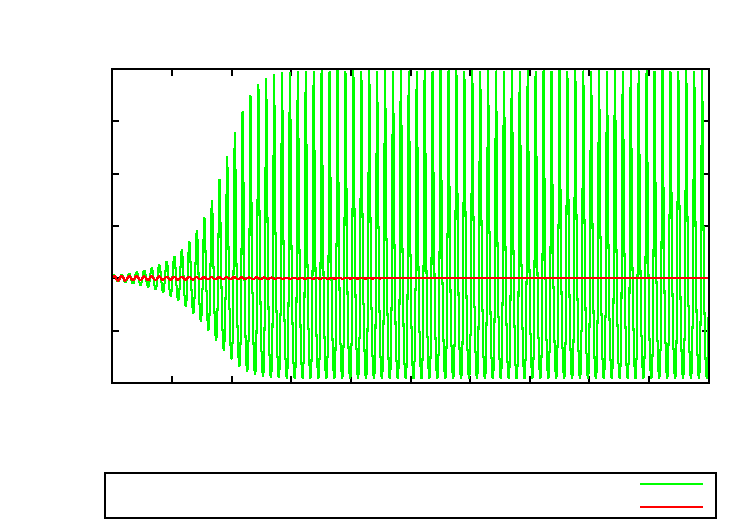
\includegraphics{a001b099uv1ER}}%
    \gplfronttext
  \end{picture}%
\endgroup
}
   \caption{Unterschiedliche Algorithmen im Vergleich}
   \label{fig:stabi}
 \end{figure}


\section{Mögliche Verbesserungen}
Als zusätzliche Verbesserung des Runge-Kutta-Algorithmus 4. Ordnung mit konstanten Zeitschritten wäre es möglich, die Zeitschritte je nach Zeitpunkt unterschiedlich zu wählen.
Es ist z.B. wichtig, wenn sich die Funktion schnell ändert, möglichst kleine Schritte zu machen.
Ändert sich jedoch wenig, so ist eine kleine Schrittweite nur rechenintensiv und trägt nur unwesentlich zu einer genaueren Berechnung bei.

\begin{thebibliography}{1000}

\bibitem{scientificcomp} 
	\textsc{J. Pitt-Francis and J. Whiteley} (2012): \emph{Guide To Scientific Computing in C++},
	1. Auflage, Springer London

\end{thebibliography}

\end{document}
